\chapter{Projektbeskrivelse}

\section{Projektgennemførelse}\label{Projektgennemfoerlse}
Projektet startede med, at der blev lavet en tidsplan, som var mulig at ændre undervejs, dog med faste deadlines, som skulle overholdes. De forskellige deadlines lagde op til, at der kunne arbejdes efter udviklingsmodeller, som er beskrevet nærmere i metodeafsnittet \ref{Metode}.\\ \\
Tidsplanen blev sidenhen ført mere detaljeret ind i projektstryringsværktøjet Scrum. Scrum blev benyttet til at holde overblikket over manglende opgaver, igangværende opgaver og afsluttede opgaver. \\
Gruppens seks medlemmer blev fra start delt op i to undergrupper, én med hovedfokus på hardware udvikling, og én med hovedfokus på software udvikling. Dog blev de basic delene til projektet, som kravspecifikation og case udvalgt samlet. Scrum er her også et godt værktøj til at bevare overblikket over de to gruppers individuelle opgaver.\\ \\
Fra start blev der aftalt et ugentlig møde, med vejleder og de to grupper som medvirkende parter. På denne måde blev alle parter holdt opdateres på udviklingsprocessen, især grupperne imellem, men også vejleder. Sidst i forløbet, under test af diverse dele af systemet, blev grupperne samlet og testene blev udarbejdet i fællesskab.\\ \\
Projektet er gennemført ved udarbejdelse af en samarbejdsaftale, herunder udvælgelse af en projektleder, som i tilfælde af uoverensstemmelse havde den afgørende stemme. 

\section{Metode} \label{Metode}
\subsection{Ase-modellen}
Den primære udviklingsmodel, der er benyttet i dette projekt, er ASE modellen. ASE modellen er en udviklingsmodel, der tager udgangspunkt i use cases. 
\begin{figure}[H]
	\centering
	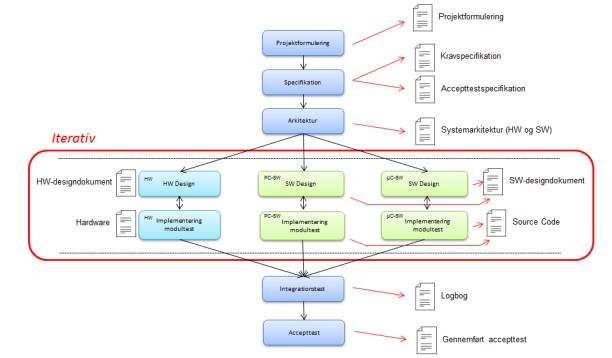
\includegraphics[width=1\textwidth]{Figurer/Metode/ASEmodellen}
	\caption{Projektmodel illustreret med de faser som projektet gennemløber\protect\footnotemark}
	\label{ASEmodel}
\end{figure}
\footnotetext{Fra \textit{"Vejledning til udviklingsprocessen for projekt 2"}}


Modellen er opbygget sådan, at udviklerne benytter vandfaldsmodellen (se afsnit \ref{Vandfald}) til at fastlægge en opgaveformulering, kravspecifikation og systemarkitektur, for derefter at designe og implementere de enkelte moduler i iterationer. \\ Ud fra projektformuleringen specificeres kravspecifikationen som en række use cases. Use cases er et værktøj, der beskriver diverse aktørers interaktion med systemet. Ved at definere kravspecifikationen ud fra use cases, opnås et overblik over hvilke krav, der stilles til systemets endelige funktionalitet.\\ \\ Ud fra kravspecifikationen kan systemets accepttest udarbejdes. Efter kravspecifikationen er fastlagt, udarbejdes systemarkitekturen.\\ I systemarkitekturen uddeles systemets funktionalitet i moduler og deres grænseflader til resten af systemet bestemmes. Ud fra systemarkitekturen designes systemet ved at nedbryde det efter funktionalitet, som kan bindes til både hardware og software.
\subsection{Vandfald}\label{Vandfald}
Denne metode bygger pa at gøre en hel fase af arbejdet færdigt før den næste startes. Grafisk ser det ud som på figur \ref{Vandfaldsmodel}: \\

\begin{figure}[H]
	\centering
	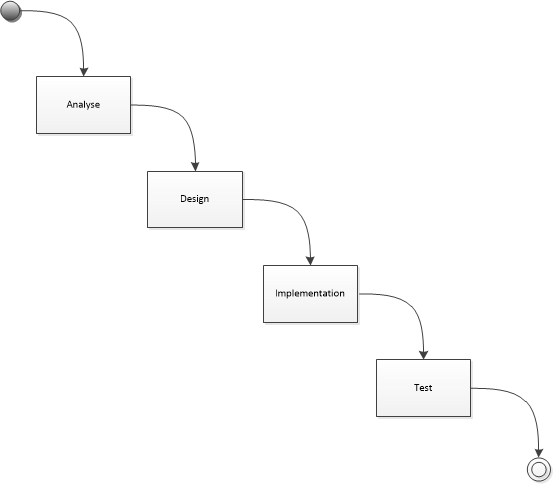
\includegraphics[width=0.8\textwidth]{Figurer/Metode/Vandfald}
	\caption{Vandfaldsmodel}
	\label{Vandfaldsmodel}
\end{figure}
Projektet starter med en analyse, og så videre med de andre faser - design, implementering og test. Det er altså hele systemet, der arbejdes igennem i hver fase, og vandfaldet symboliserer, at der kun arbejdes i en retning, altså man kan ikke gå imod strømmen. Metoden benyttes, når opgaven er veldefineret og velkendt. \\
Projekt forløbet skal have en kort varighed, dvs. mindre end ca. 4 måneder, under velkendte forhold med hensyn til udviklings- og testmiljø, udviklingsmetodik, platforme etc. \cite{Projektledelse}

\subsection{V-model}
V-modellen er en model, hvor testen planlægges parallelt med udviklingen. Accepttesten planlægges detaljeret efter kravnalysen, altså kravspecifikationen, systemtest planlægges detaljeret efter system design, og integrationstesten planlægges detaljeret efter arkitektur design fasen. Unit/modul testen ligger dog uændret i forhold til den traditionelle strategi.
\begin{figure}[H]
	\centering
	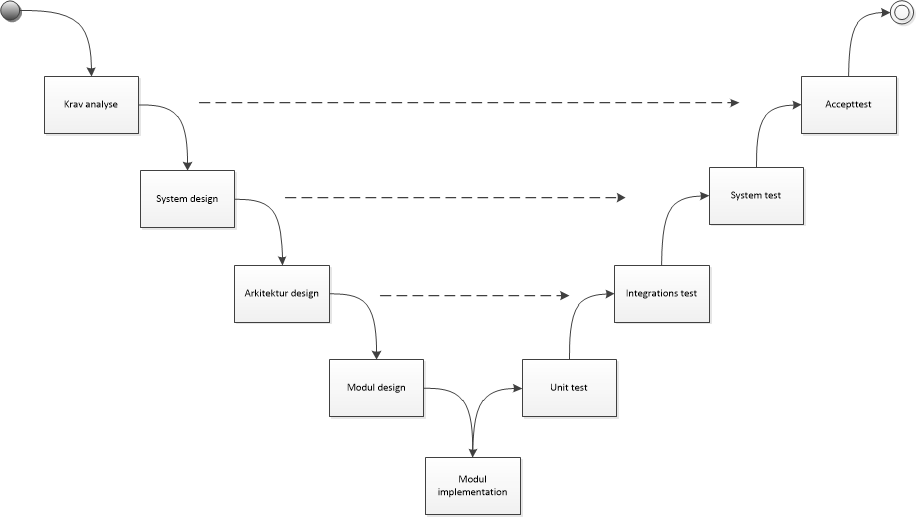
\includegraphics[width=1\textwidth]{Figurer/Metode/Vmodel}
	\caption{V-model}
	\label{Vmodel}
\end{figure}
Testens praktiske udførelse er altså uændret i forhold til Ase-modellen og Vandfaldsmodellen, dvs. den ligger sidst i forløbet. Det betyder at testfaserne planlægges modsat den rækkefølge, de udføres i. Den største forskel for testerne er, at planlægningen baseres på de tidlige modeller af systemet, ikke på det færdige system. \\
 V-modellen udvides desuden med reviews og deadlines (se afsnit \ref{Projektgennemfoerlse}).

\section{Specifikation og analyse}



\chapter{Arkitektur}
I det følgende afsnit beskrives arkitekturen for systemet. Systemarkitekturen fungerer her som udviklingsramme for videre design og implementering. Her bliver systemets funktionalitet 
nedbrudt til overordnede moduler. \\
   Arkitekturen for projektet er foretaget i to dele - en hardware arkitektur og en software arkitektur. Arkitekturen beskriver opbygningen af systemet i form af diagrammer.  
   
\section{Software arkitektur}\label{Software arkitektur}
   I software designet er der udarbejdet en domæne model, der giver et overblik over hele systemet.
   
 \begin{figure}[H]
	\centering
	\includegraphics[width=1\textwidth]{Figurer/ISE/Domaenemodel}
	\caption{Domænemodel}
	\label{domaenemodel}
\end{figure}

I domæne-modellen er relationerne mellem aktørerne og systemets dele beskrevet med pile og vejledende tekster - dette skulle gerne give et større overblik over systemets funktionalitet. \\ 
En domænemodel beskriver dog ikke, hvilken rækkefølge de forskellige handlinger sker i, og derfor er der udarbejdet sekvensdiagrammer for hver use case for systemet, som skal beskrive dette.\\
Nedenfor på figur \ref{sekvensdiagram} ses sekvensdiaframmet for use casen "Mål blodtryk":

\begin{figure}[H]
	\centering
	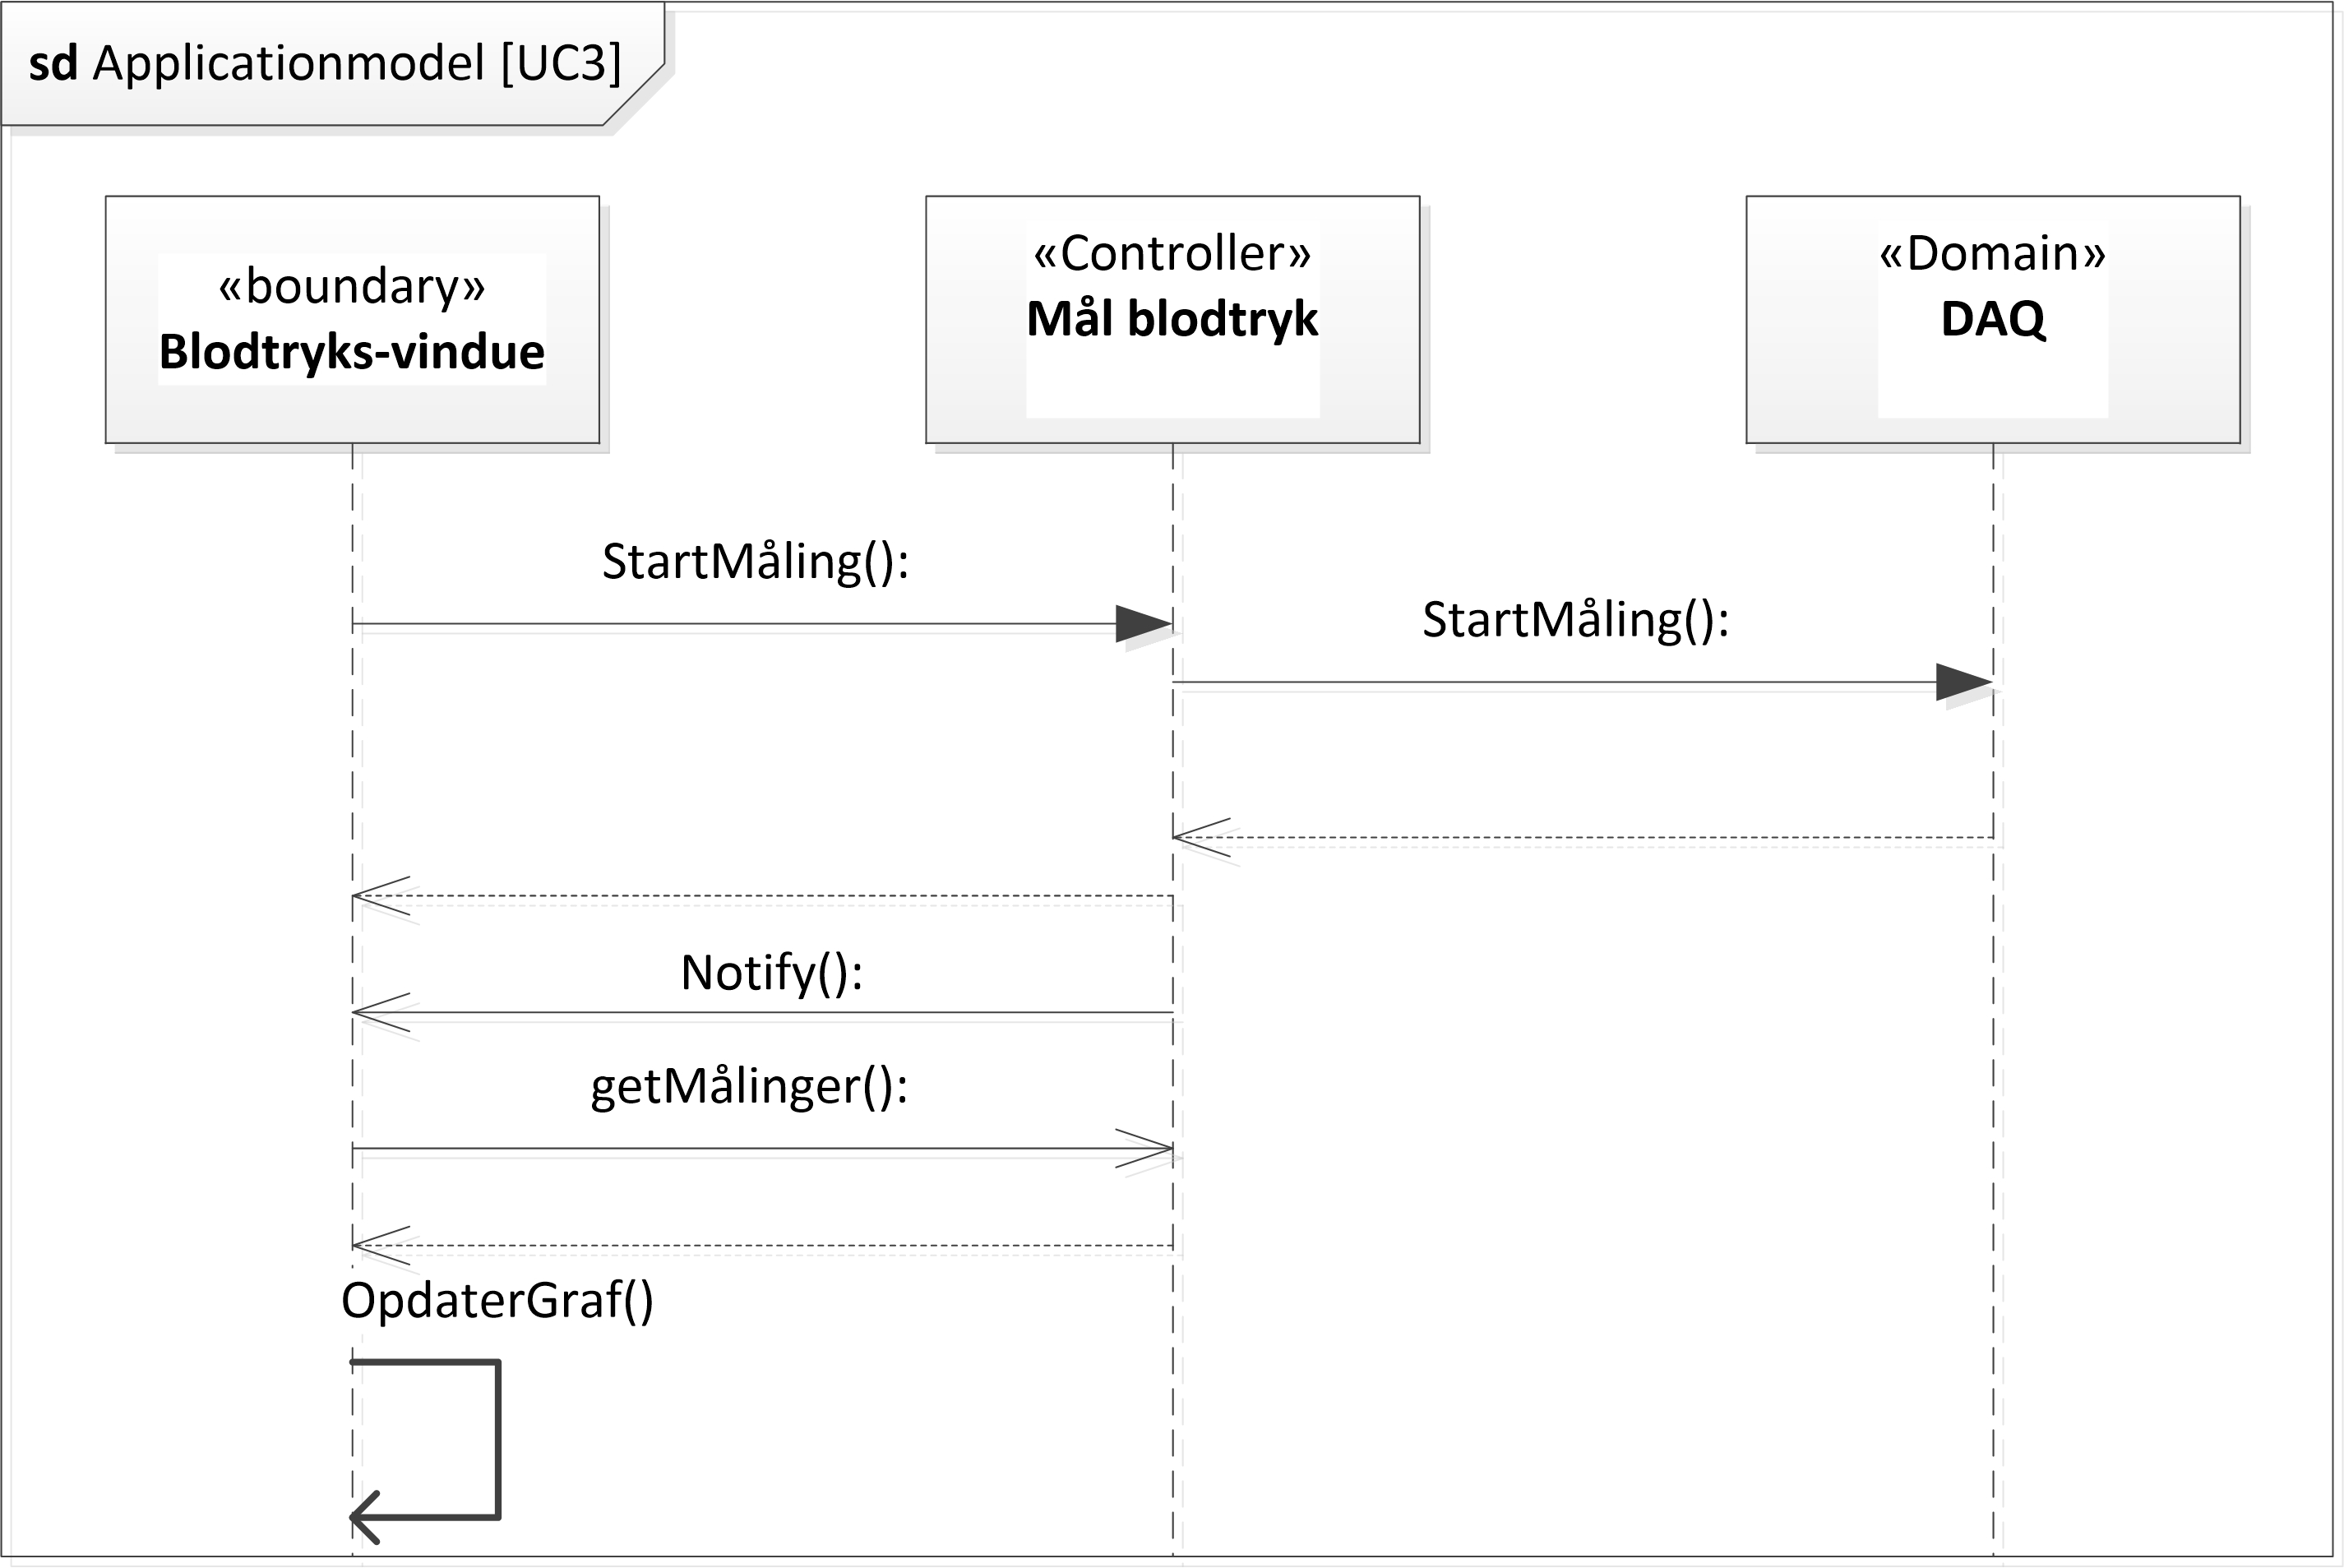
\includegraphics[width=1\textwidth]{Figurer/ISE/sdAppModelUC3}
	\caption{Sekvensdiagram UC3}
	\label{sekvensdiagram}
\end{figure}

Figur \ref{sekvensdiagram} viser hvordan brugeren interagerer med brugergrænsefladen ved at starte blodtryksmålingen. Herefter bliver metoden til at starte blodtryksmålingen kaldt ned gennem logik- og datalag hvor efter målingen vises i en graf på brugergrænsefladen. Grafen bliver hele tiden opdateret med nye målinger.\\
Ud fra dette kan det ses hvordan brugerens interaktion med brugergrænsefladen sætter gang i metoder i software programmet. Skevensdiagrammet giver altså et overblik over hvordan softwaren er bygget op.\\
Sekvensdiagrammerne for de øvrige use cases kan ses i dokumentationen afsnit \textbf{Afsnit i dokumentation}
  
 \subsection{SysML}
 I beskrivelsen af systemarkitekturen og det detaljerede design for det færdige produkt, er der anvendt SysML. SysML stammer oprindeligt fra UML, men UML er hovedsagligt centreret omkring udvikling af software systemer. Da det udviklede system både består af hardware og software, er der valgt SysML til beskrivelsen af arkitekturen.\\
Valget af SysML grunder også i, at det giver en god formidling af systemet - dette giver udviklerne et større overblik. Samtidig er det også let for en udenforstående at sætte sig ind i systemets kunnen.\\

I dette projekt er der benyttet struktur- og adfærdsdiagrammer til at specificere og dokumentere systemet. Som strukturdiagram er der anvendt et blok definitions diagram (bdd) samt interne blok definitions diagramm (ibd).\\
Der er anvendt adfærdsdiagrammer i form af sekvensdiagrammer i dette projekt. Disse diagrammer er velegnet til sekventielt at beskrive den logiske funktionalitet i systemet. Softwaren er opbygget ud fra sekvensdiagrammer beskrevet i arkitektur afsnittet (afsnit \ref{Software arkitektur}).

\chapter{Design, implementering og test}


\subsection{Implementering}
Efter komponentudregningen, byggede gruppen de to hardware blokke op. Gruppen valgte at bygge forstærkeren og filteret seperat, grundet pladsmangel og sammenhæng.\\

\begin{figure}[H]
	\centering
	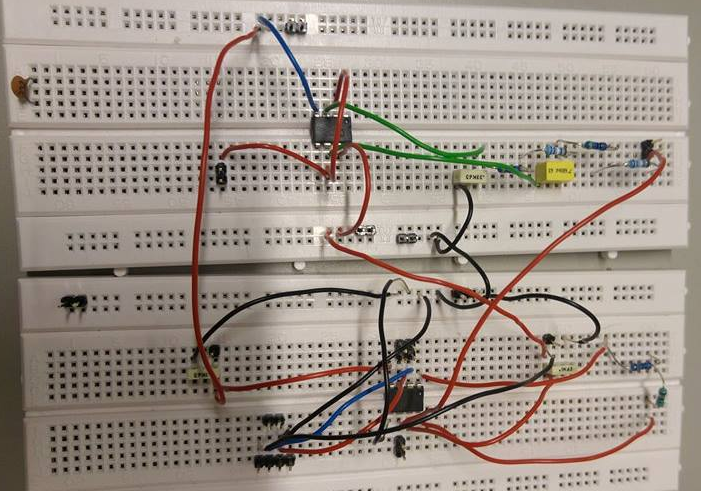
\includegraphics[width=1\textwidth]{Figurer/Hardware/samletopstilling}
	\caption{Opstilling af forstærker og filter}
	\label{samletopbygning}
\end{figure}

Grundet mangel på præcise modstande, bedømte gruppen at det var bedst at bygge modstandende i forholdsvist filteret og forstærkeren, op i to, så gruppen kunne komme så tæt på den ønskede modstandsværdi som muligt. \\
For forstærkeren, blev styklisten som vist på tabel \ref{forsttabel}.


\begin{table}[H]
\centering
\begin{tabular}{lllll}
\textbf{Komponent} & \textbf{Antal} & \textbf{Type}  &  &  \\ \cline{1-3}
Modstand           & 1              & 120 $\Omega$   &  &  \\ \cline{1-3}
Modstand           & 1              & 4.8 $\Omega$   &  &  \\ \cline{1-3}
Kondensator        & 2              & 100 nF         &  &  \\ \cline{1-3}
Instrumentationsforstærker &    1   & INA114		     &  &  \\ \cline{1-3}
\end{tabular}
\caption{Forstærkertabel}
\label{Forsttabel}
\end{table}

Grundet forskel imellem teoretiske værdier og fysiske, er R$_{gain}$ 0,51$\Omega$ mindre end den skulle have været.\\

Den samlede stykliste for filteret blev som vist på tabel \ref{Filtertabel}.

\begin{table}[H]
\centering
\begin{tabular}{lllll}
\textbf{Komponent} & \textbf{Antal} & \textbf{Type}  &  &  \\ \cline{1-3}
Modstand           & 2              & 6.2 k $\Omega$ &  &  \\ \cline{1-3}
Modstand           & 2              & 470 $\Omega$   &  &  \\ \cline{1-3}
Kondensator        & 1              & 680 nF         &  &  \\ \cline{1-3}
Kondensator        & 1              & 330 nF         &  &  \\ \cline{1-3}
Operationsforstærker &    1         & OP27G          &  &  \\ \cline{1-3}
\end{tabular}
\caption{Filtertabel}
\label{Filtertabel}
\end{table}

I det analoge filter, er kondensatoren, C$_1$, i praksis 3,2 nF mindre end  beregnet. Desuden er de to identiske modstande, R$_1$ og R$_2$, som i praksis er 17$\Omega$ mindre end teorien foreskriver.\\
Gruppen vurderede at afvigelserne var forholdsvidst små, og derfor er der valgt at se bort fra dem. For modstandende er der desuden 1 procents usikkerhed, hvilket betyder man alligevel ikke kan være helt sikker på komponentværdien.\\
En reel cutoff frekvens blev herefter udregnet af gruppen. Denne kan ses udregnet på figur \ref{cutoff}.


\begin{align}
f_{c} = \frac{1}{2\pi \sqrt{R_{1}C_{1}R_{2}C_{2}}} = \frac{1}{2\pi \sqrt{6687 \cdot 333,2\times 10^{-9} \cdot 6687 \cdot 680\times 10^{-9}}} = 50,37 Hz
	\label{cutoff}
\end{align}
%\caption{Udregning af den reelle cutoff frekvens}



\subsection{Test}


\section{Resultater og diskussion}


\section{Opnåede erfaringer}


\section{Fremtidigt arbejde}
